\documentclass[tikz]{standalone}

\usepackage[T1]{fontenc}
\usepackage[english]{babel}

\usepackage{standalone}

\usepackage{tikz}
\usetikzlibrary{calc}

\begin{document}
    \begin{tikzpicture}
        \node (recon) {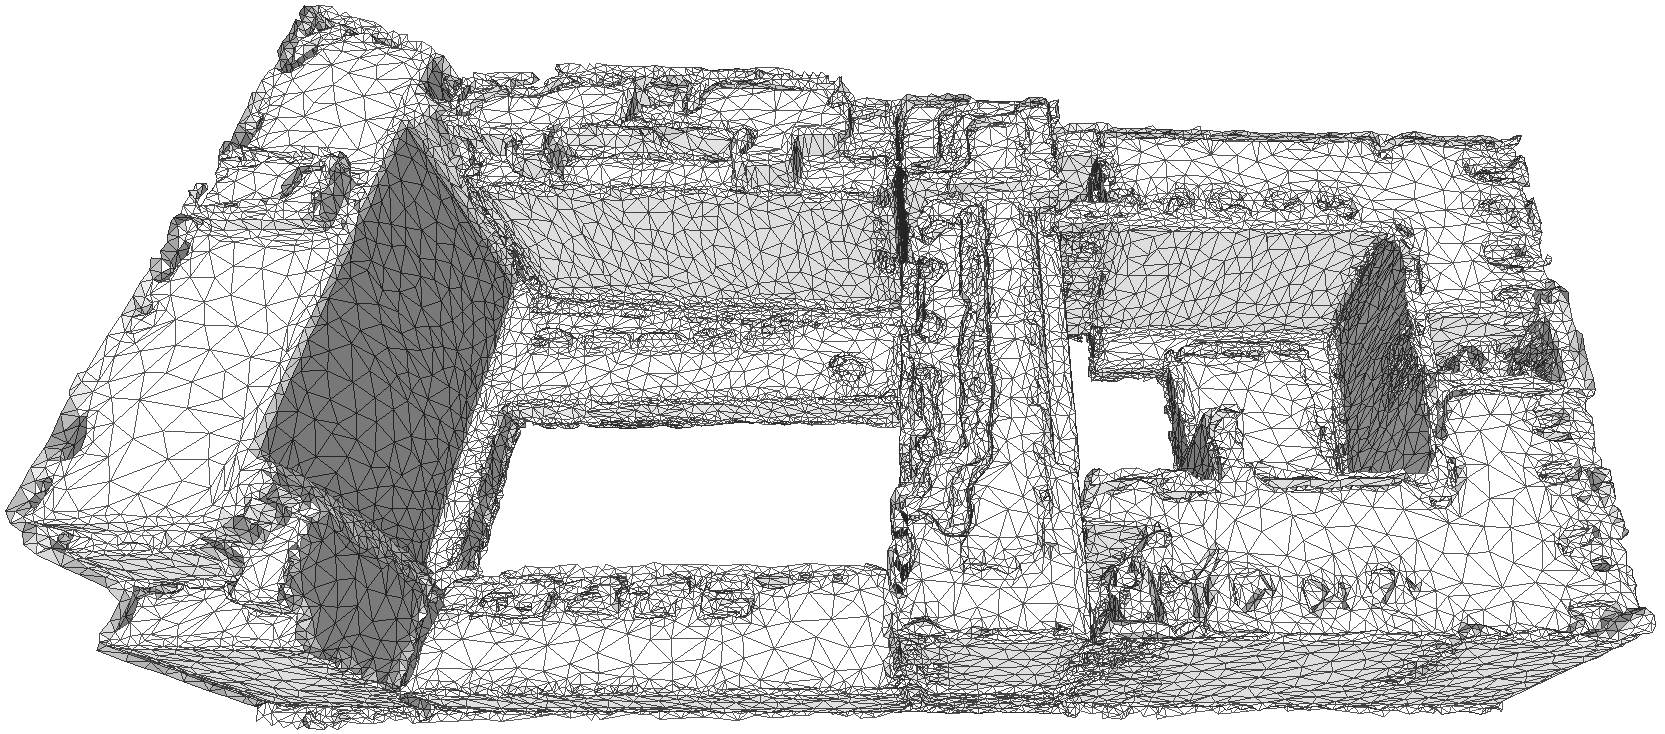
\includegraphics[height=4cm]{images/introduction/difference_mesh_model/bercy_building_mesh_1_e5}};
        \path (recon.east) + (.5, 0) node[anchor=west, visible on=<3->] (model) {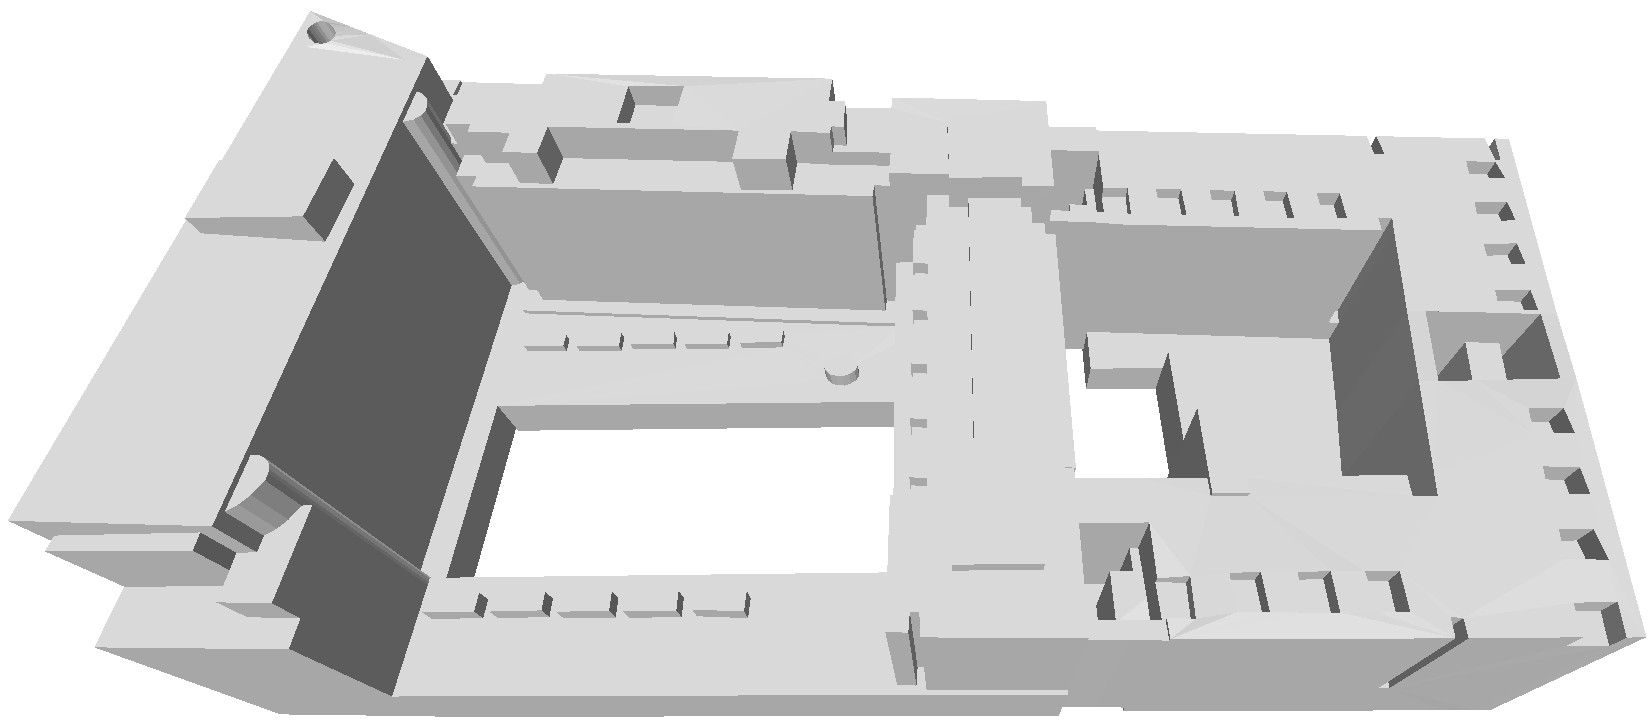
\includegraphics[height=4cm]{images/introduction/difference_mesh_model/ground_truth}};
        \path[draw, blue, line width=0.1mm, <->] ($(recon.south) + (-3, 0)$)  -- ($(recon.south) + (3.7, 0)$) node[midway, below] {\tiny \SI{139}{m}};
        \path[draw, blue, line width=0.1mm, <->, visible on=<3->] ($(model.south) + (-3, 0)$)  -- ($(model.south) + (3.7, 0)$) node[midway, below] {\tiny \SI{139}{m}};

        \draw[<->, very thick, visible on=<4->] (recon.east) -- (model);
    \end{tikzpicture}
\end{document}
